\section{Spring 2006}

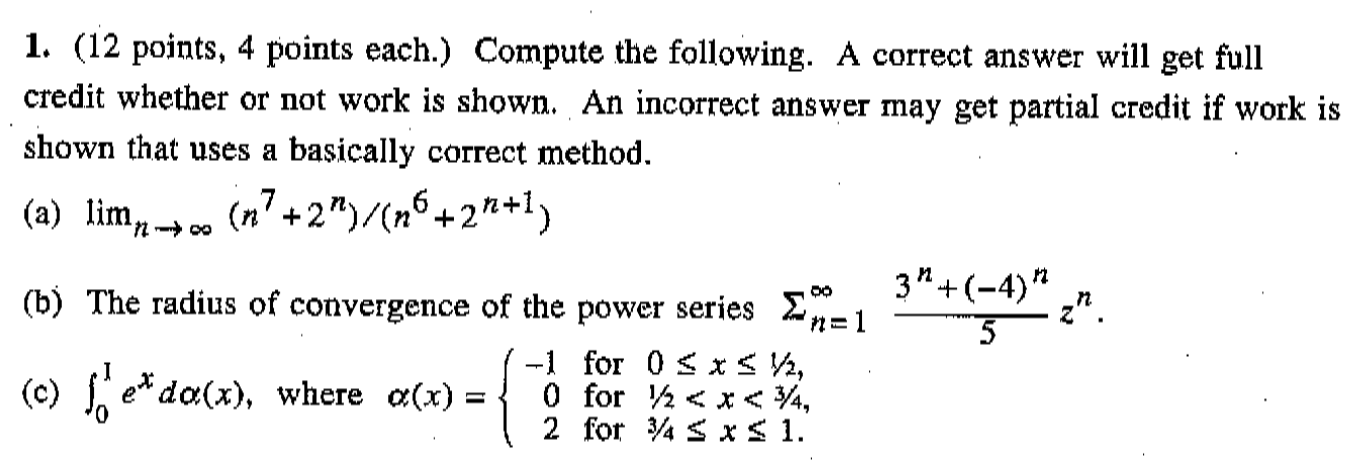
\includegraphics[width=400pt]{img/analysis--berkeley-104-final--spring-2006-6245.png}

\begin{enumerate}[label=(\alph*)]
\item
\begin{align*}
    \lim_{n\to\infty} \frac{n^7 + 2^n}{n^6 + 2^{n+1}}
   = \lim_{n\to\infty} \frac{1}{2}
   = 1/2 \checkmark
\end{align*}
\item Converges if $|4z| < 1$, i.e. $z \in (-1/4, 1/4)$. \checkmark
\item $1 - e^{1/2} + 2(e - e^{3/4})$ nope $e^{1/2} + 2e^{3/4}$
\end{enumerate}


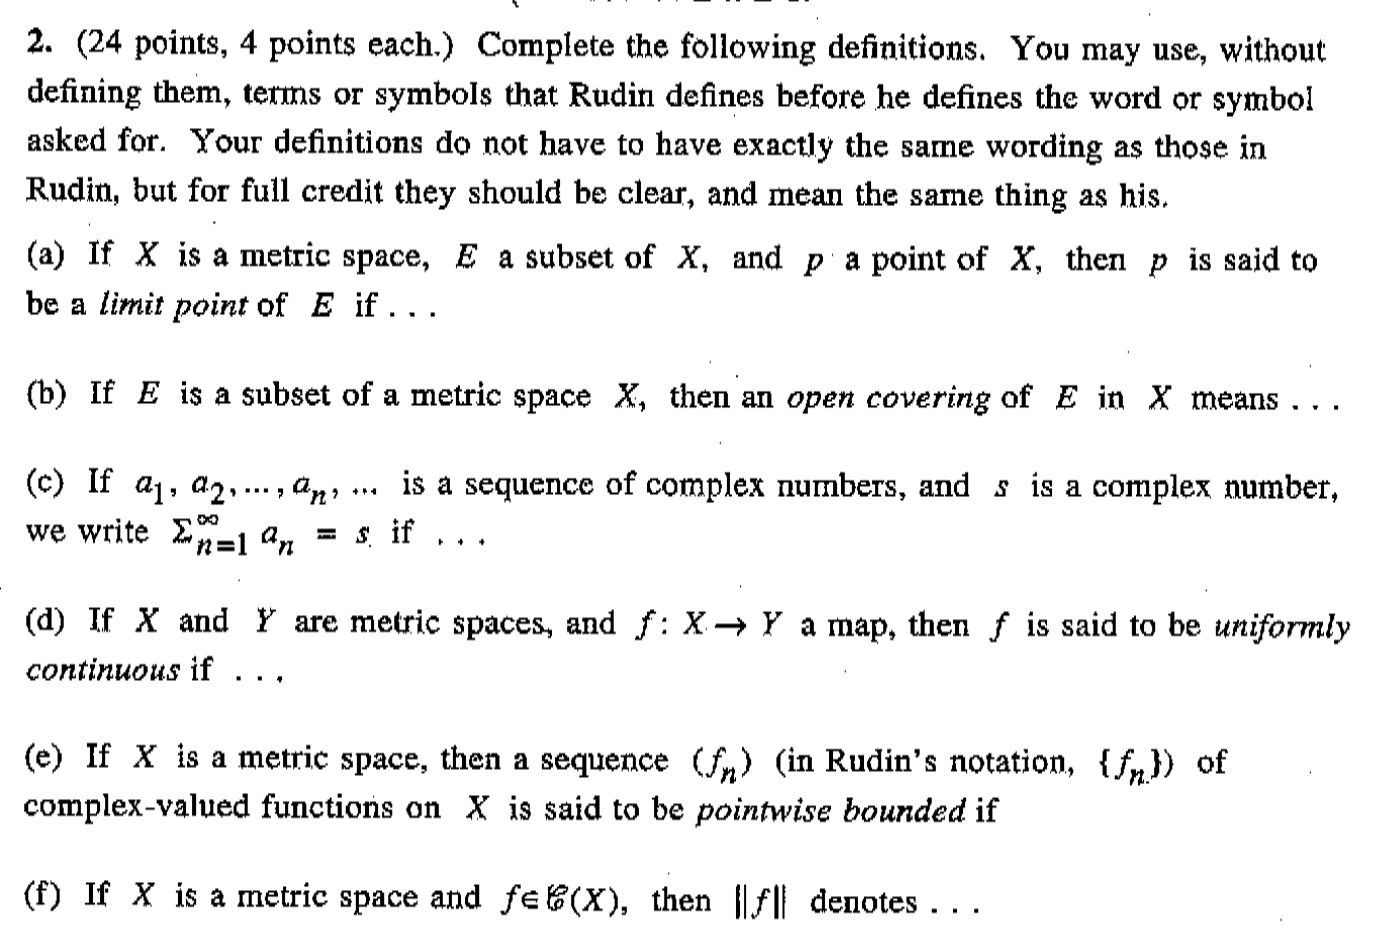
\includegraphics[width=400pt]{img/analysis--berkeley-104-final--spring-2006-d466.png}

\begin{enumerate}[label=(\alph*)]

\item $p \in X$ is a limit point of $E \subseteq X$ if there exists a sequence $e_1, e_2, \ldots$ with
  limit $p$, where $e_i \in E$ for all $i$.

  ...if every neighborhood of $p$ contains a point $q \neq p$ such that $q \in E$.

\item An open covering in $X$ of $E \subseteq X$ means a collection of open sets $S_1, \ldots, S_n$ such
  that each $S_i \subseteq X$ and $E \subseteq \bigcup_i S_i$.

\item We write $\sum_{n=1}^{\infty} a_n = s$ if $s$ is the limit of the sequence of partial sums, i.e.
  if $\lim_{n\to\infty} \sum_{i=1}^n a_i = s$.

\item $f$ is \defn{uniformly continuous} if for all $\epsilon > 0$ there exists $\delta > 0$ such that for all
  $x, x' \in X$ we have that $d(x, x') < \delta \implies d\(f(x) - f(x')\)| < \epsilon$. I.e., for any
  given $\epsilon$, the same $\delta$ ``works​'' at all points $x \in X$.

\item A sequence $(f_n)$ of complex-valued functions on a metric space $X$ is \defn{pointwise bounded} if for all
  $x \in X$ there exists $B$ such that for all $n$ we have $|f_n(x)| < B$.

\item If $f$ is complex-valued, continuous and bounded, then $\norm{f}$ denotes $\sup_{x\in X} |f(x)|$.

\end{enumerate}
$\checkmark$

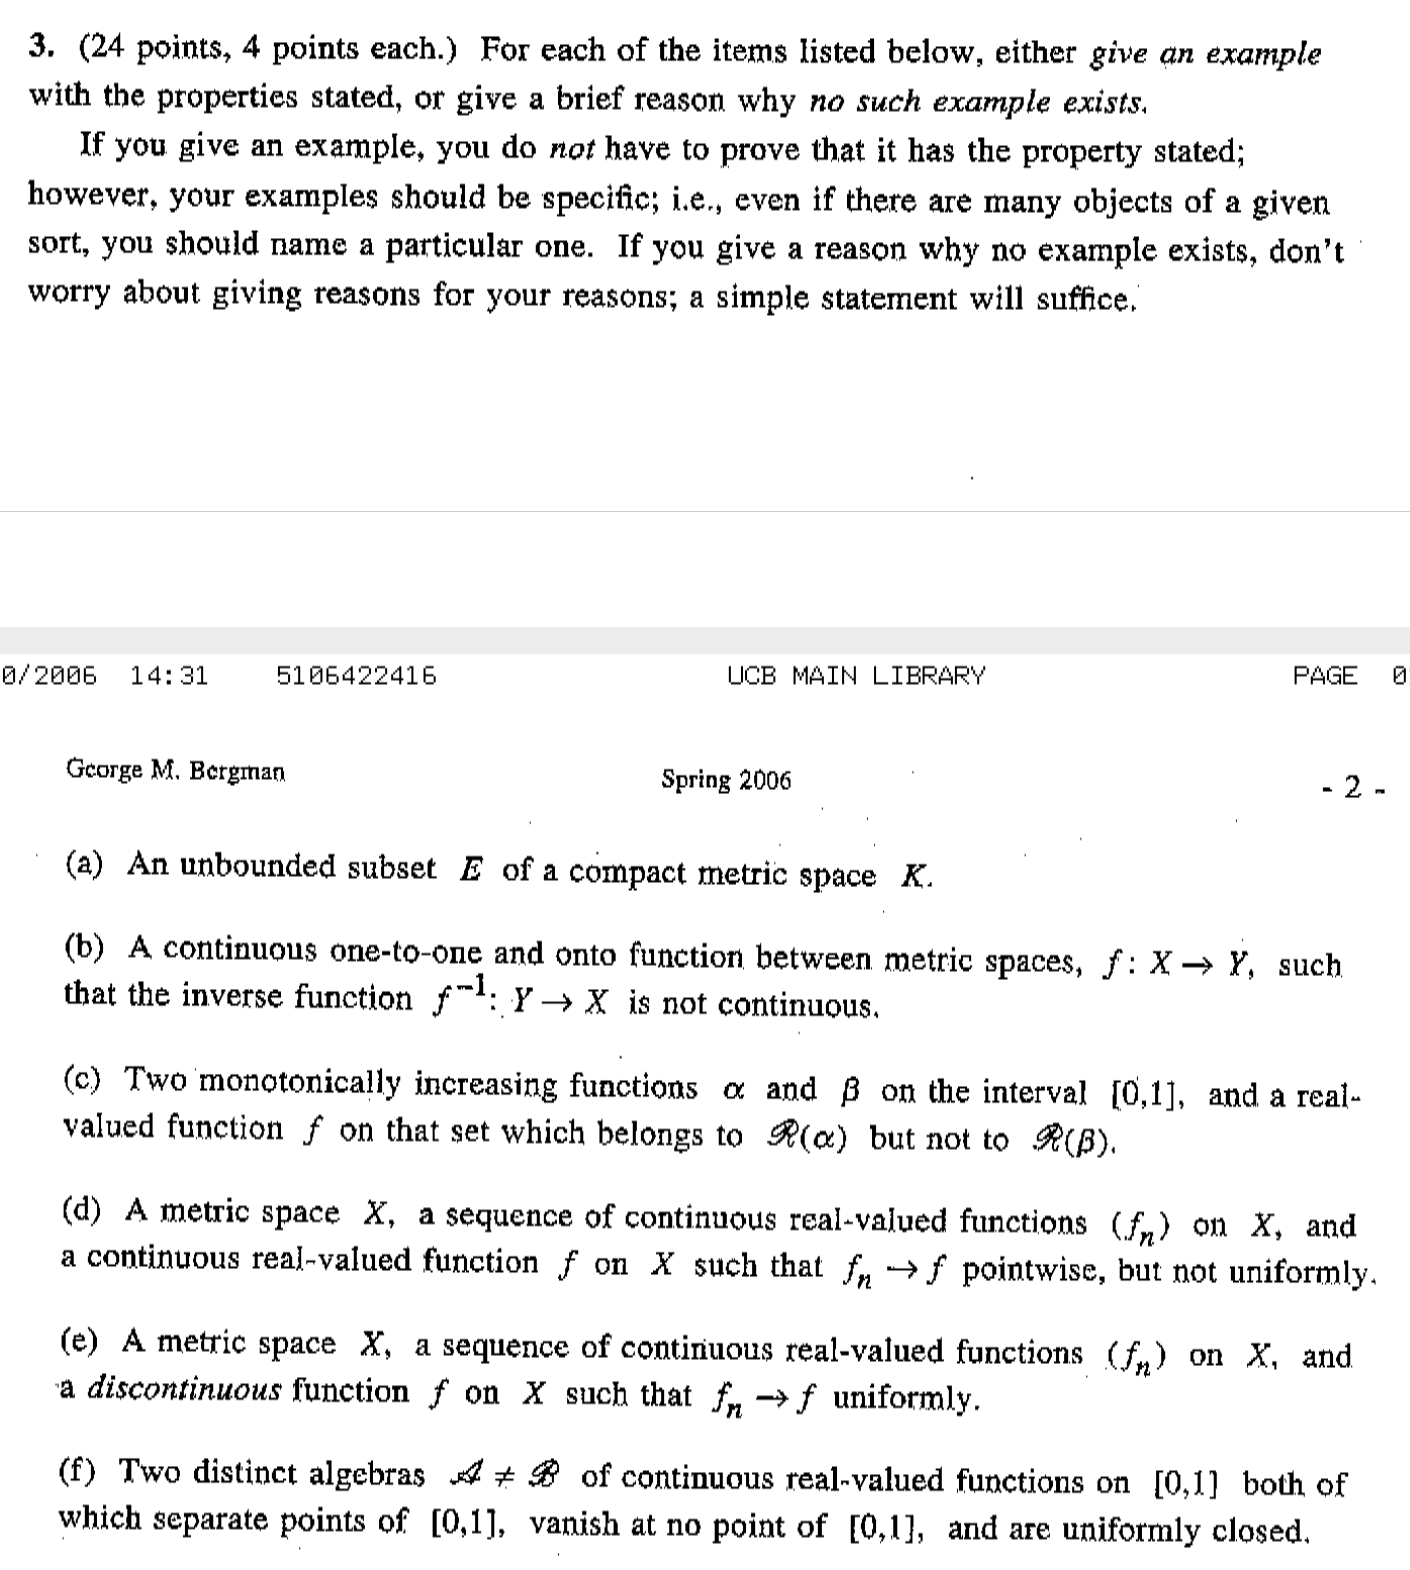
\includegraphics[width=400pt]{img/analysis--berkeley-104-final--spring-2006-71a2.png}

\begin{enumerate}[label=(\alph*)]

\item Does not exist. If metric space $K$ is compact then it is bounded, and a subset of a bounded metric space is
  bounded.

\item E.g. map $[0, 2\pi)$ to the unit circle with $f(t) = (\cos t, \sin t)$. Then the inverse $f^{-1}$ is not
  continuous at $(1, 0)$, since $f^{-1}((1, 0)) = 0$ but $\lim_{(x, y) \to (1, 0)} f^{-1}((x, y)) = 2\pi$ when
  the limit is of a sequence of points approaching $(1, 0)$ along the unit circle in the 4th quadrant.





\item [Riemann-Stieltjes integral]

\item Does not exist: a sequence of continuous functions that converges pointwise converges uniformly.

\item Does not exist: if $(f_n)$ are continuous and $f_n \to f$ uniformly then $f$ is continuous.

\item [Algebras of functions]

\item



\end{enumerate}




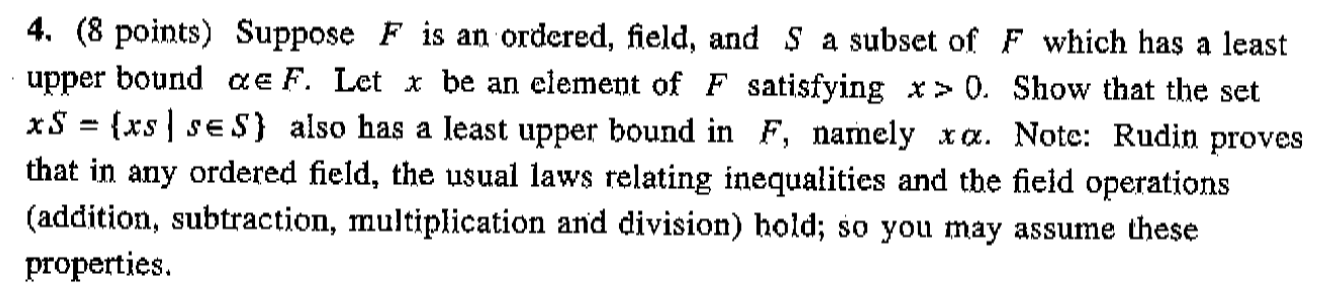
\includegraphics[width=400pt]{img/analysis--berkeley-104-final--spring-2006-2fa6.png}



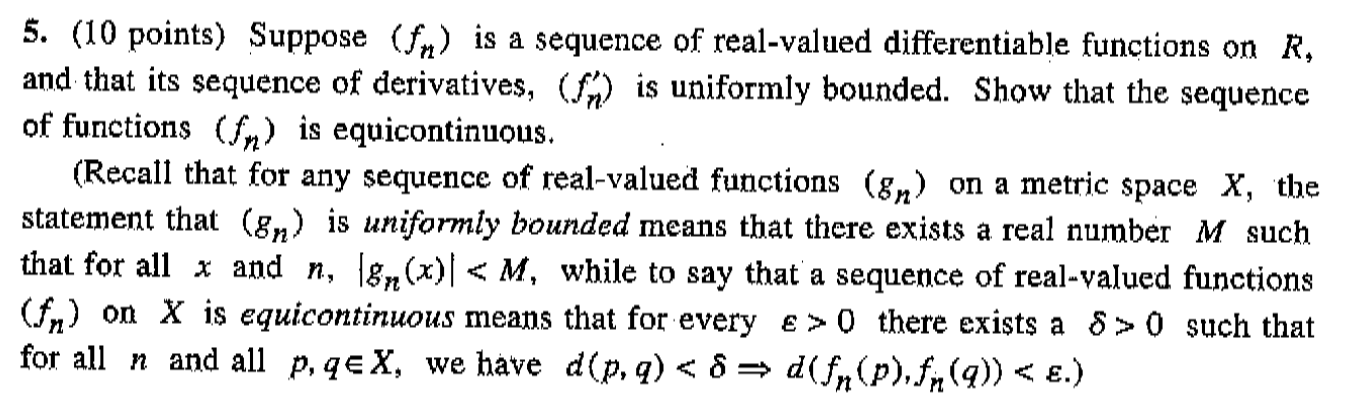
\includegraphics[width=400pt]{img/analysis--berkeley-104-final--spring-2006-0a2d.png}



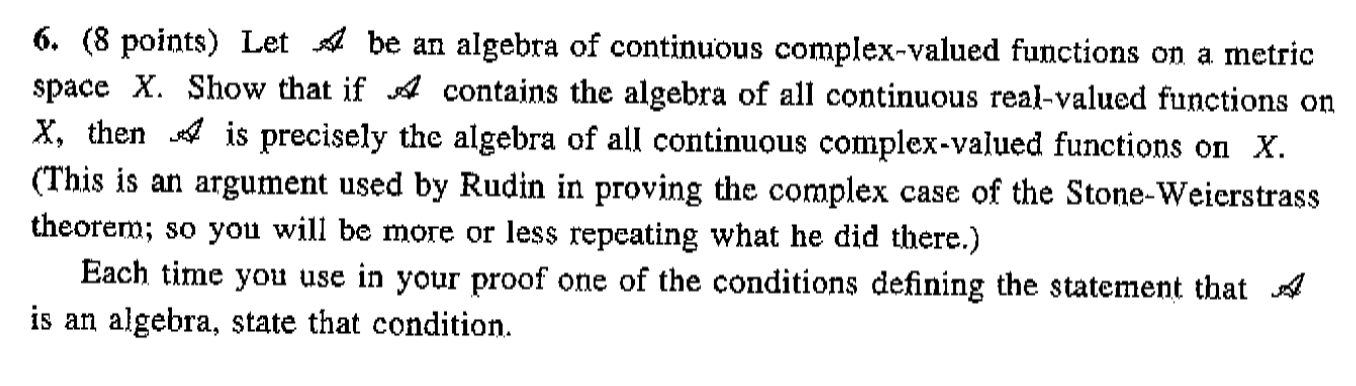
\includegraphics[width=400pt]{img/analysis--berkeley-104-final--spring-2006-3cc8.png}




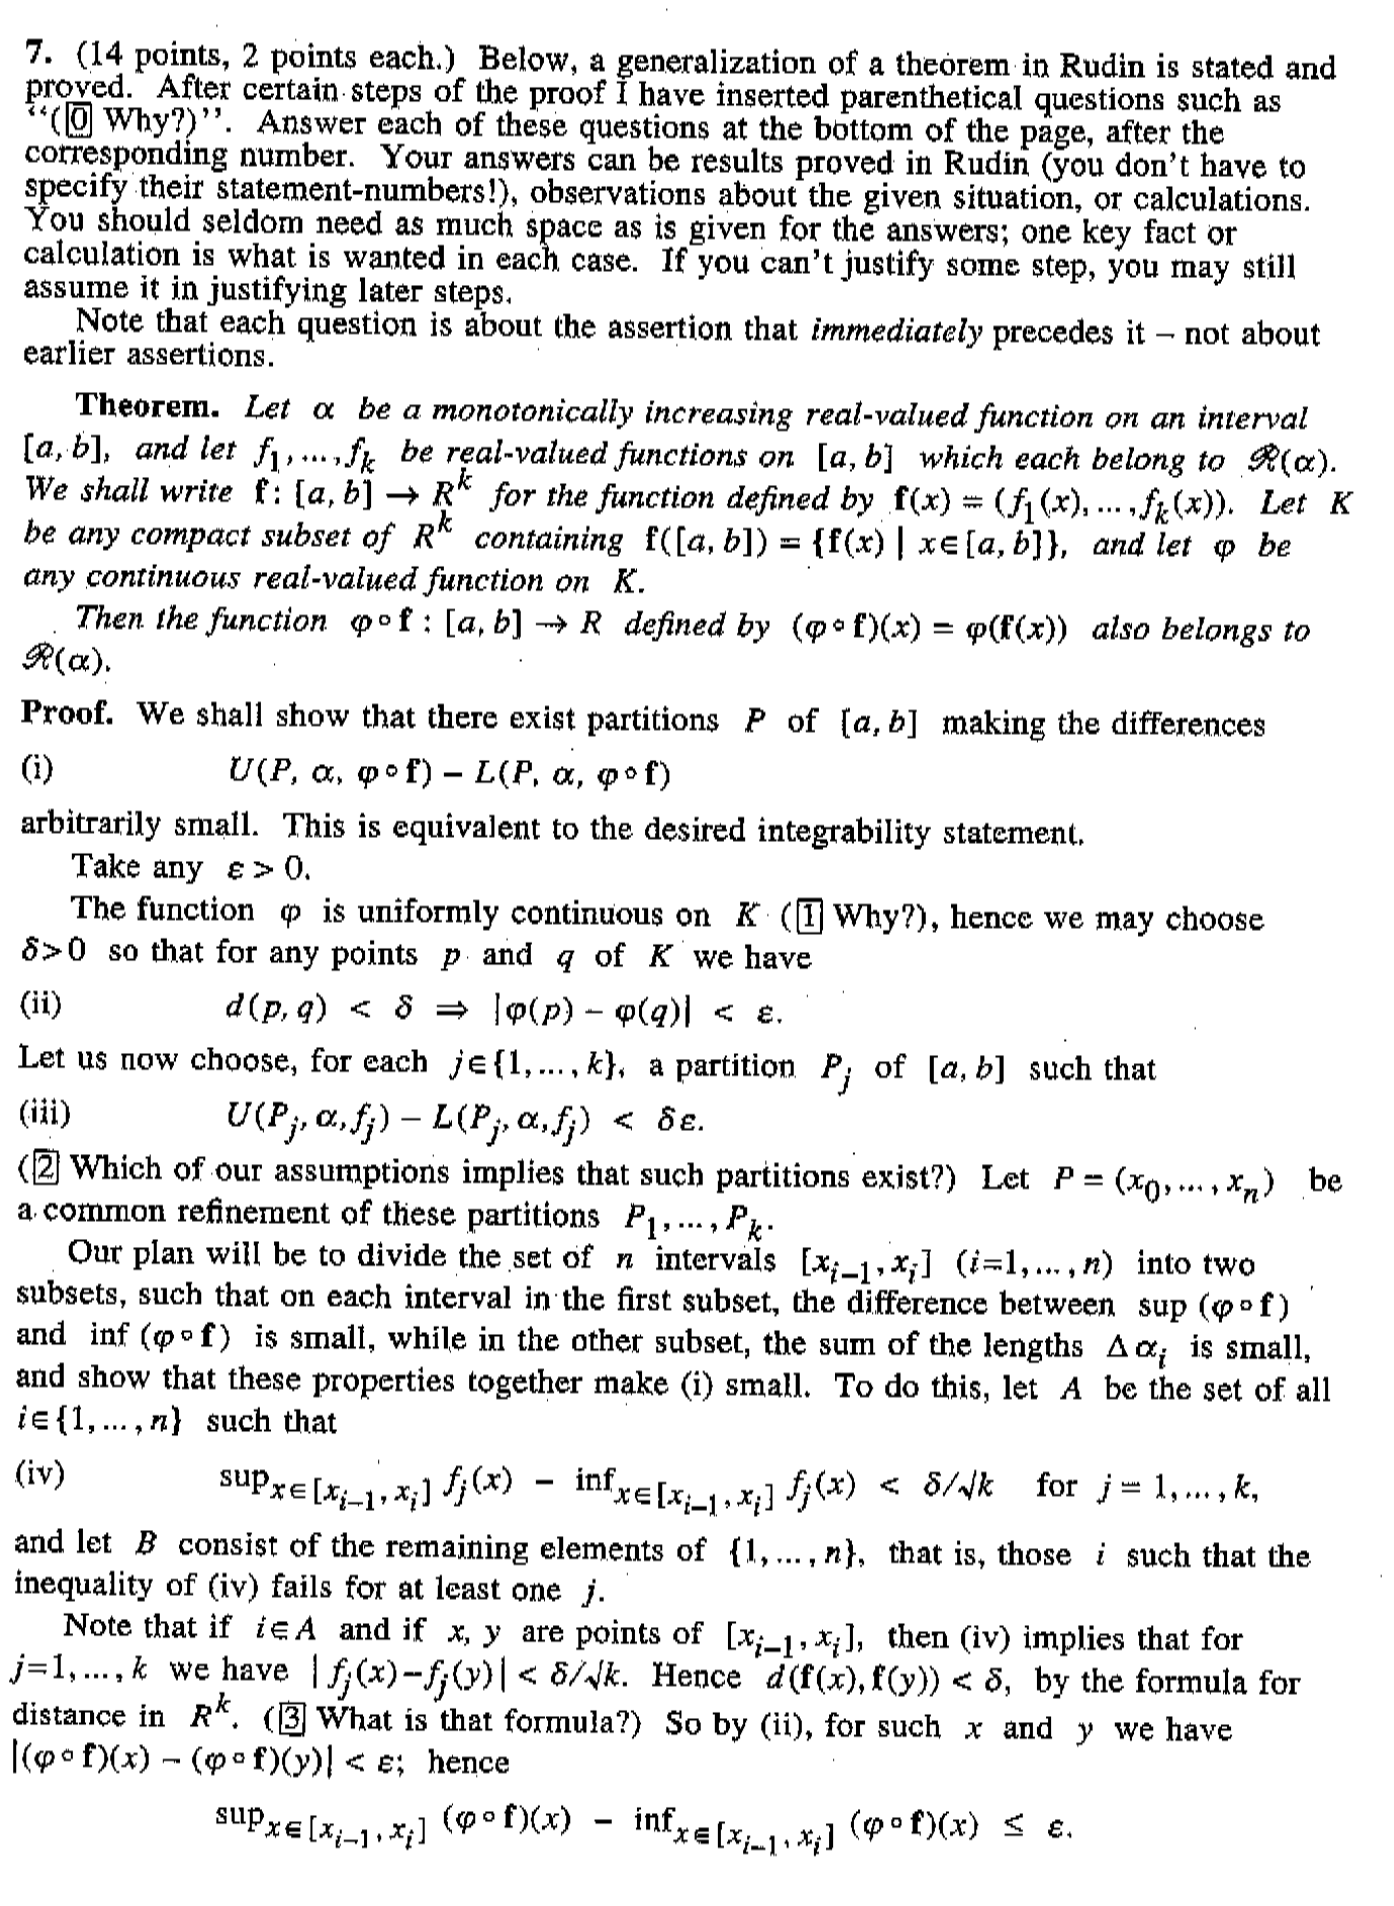
\includegraphics[width=400pt]{img/analysis--berkeley-104-final--spring-2006-b835.png}

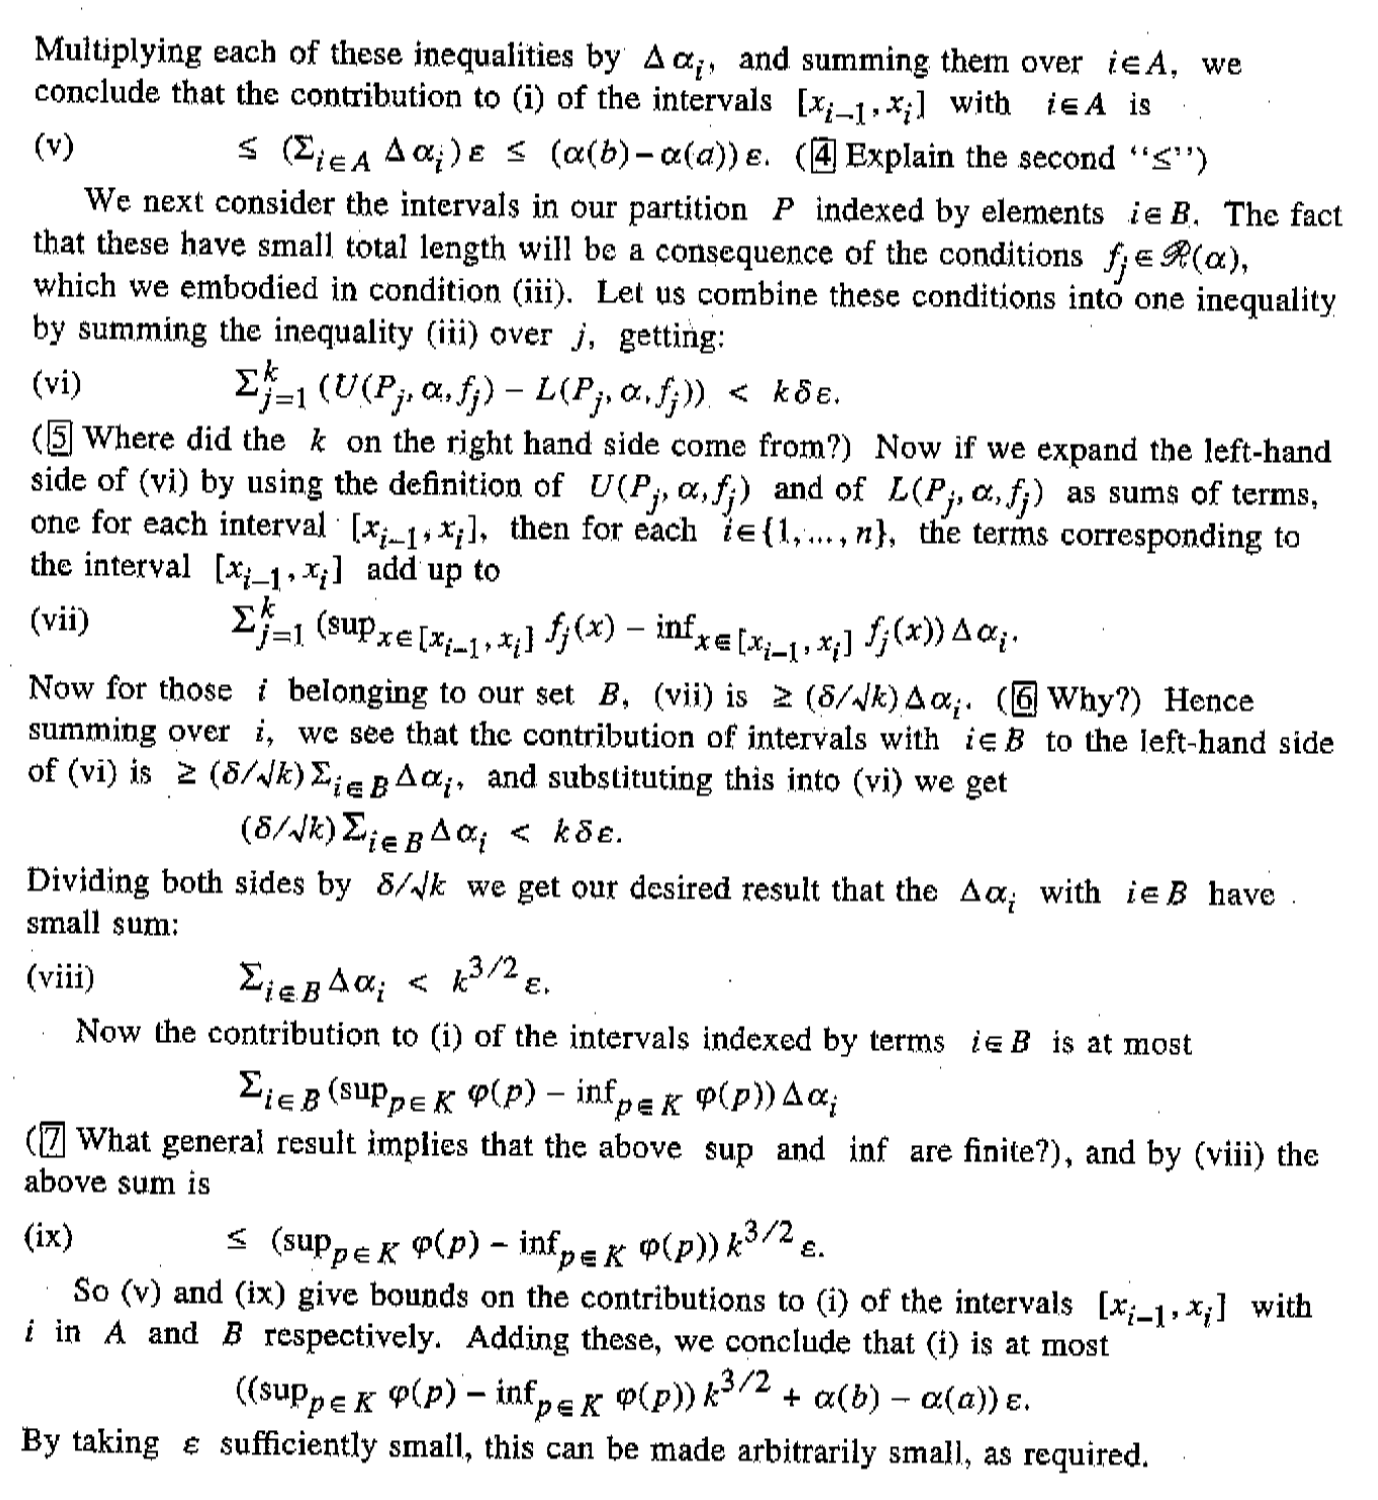
\includegraphics[width=400pt]{img/analysis--berkeley-104-final--spring-2006-9a48.png}




\section{2013}

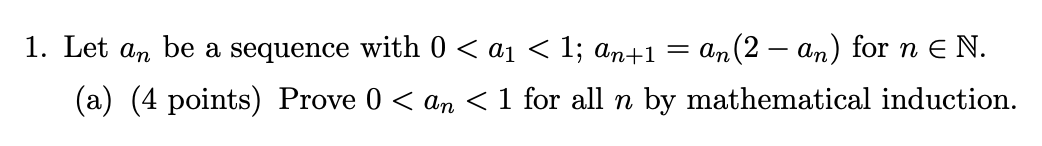
\includegraphics[width=400pt]{img/analysis--berkeley-104-final-1f72.png}

Suppose $0 < a_k < 1$. Then $a_{k+1} = a_k(2 - a_k) = 2a_k - a_k^2 = a_k + a_k(1 - a_k) < 1$.
Since $0 < a_1 < 1$ we have that $0 < a_n < 1$ by induction.


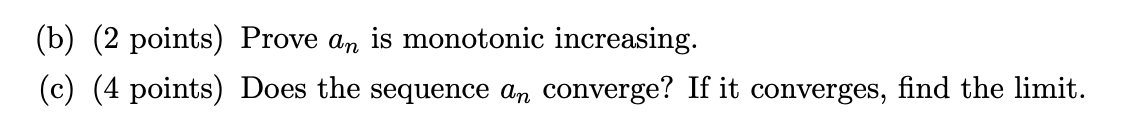
\includegraphics[width=400pt]{analysis--berkeley-104-final-630e.png}

The difference between successive terms is $a_{k+1} - a_k = 2a_k - a_k^2 - a_k = a_k(1 - a_k) > 0$, therefore
the sequence is monotonic increasing.

Since the sequence is bounded above, and monotonic increasing, it converges.

\begin{proof}
  Let $(a_n)$ be monotonic increasing and bounded above by $B$. We claim that there exists $L$ satisfying the
  following: for all $\epsilon > 0$ there exists an $N$ such that $|a_n - L| < \epsilon$ for all $n > N$.

  Let $S = \sup \{a_1, a_2, \ldots\}$. $S$ exists by the completeness axiom for the real numbers,
  since $\{a_1, a_2, \ldots\}$ is bounded above. We claim that $S$ is a limit.

  Suppose for a contradiction that $S$ is not a limit. Let $\epsilon > 0$ be such that no $N$ works for
  that $\epsilon$ (such an $\epsilon$ exists by our supposition that $S$ is not a limit). Then there does not
  exist $N$ such that $a_N > S - \epsilon$, since otherwise $N$ would work for $\epsilon$. But
  then $S - \epsilon$ is a lower bound and less than the supremum, which is a contradiction.

  Therefore $(a_n)$ converges to its supremum.
\end{proof}

In the limit, $a_{n+1} \to L$ and $a_n \to L$ and we have
\begin{align*}
  L &= L(2 - L) \\
  L^2 - L &= 0 \\
  L(L - 1) &= 0.
\end{align*}
Therefore $L = 1$ since $a_1 > 0$ and the sequence is monotonic increasing.

Alternatively,
\begin{align*}
  \lim_{n\to\infty} \frac{a_{n+1}}{a_n} = \lim_{n\to\infty} 2 - a_n = 2 - \lim_{n\to\infty} a_n = 1,
\end{align*}
therefore the limit is $\lim_{n\to\infty} a_n = 1$.

\checkmark

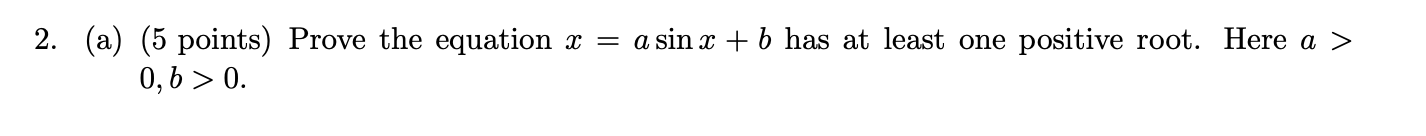
\includegraphics[width=400pt]{analysis--berkeley-104-final-ecb4.png}
\begin{proof}
  Let $g(x) = a\sin x + b$ and let $f(x) = x - g(x)$.

  Note that $f$ is continuous, that $f(0) = -b < 0$, and that the maximum value attained by $g(x)$ is $a + b$ and
  therefore that $f(a + b + 1) = a + b + 1 - g(x) > 0$. Therefore there exists $x > 0$ such that $f(x) = 0$ by
  the intermediate value theorem.
\end{proof}

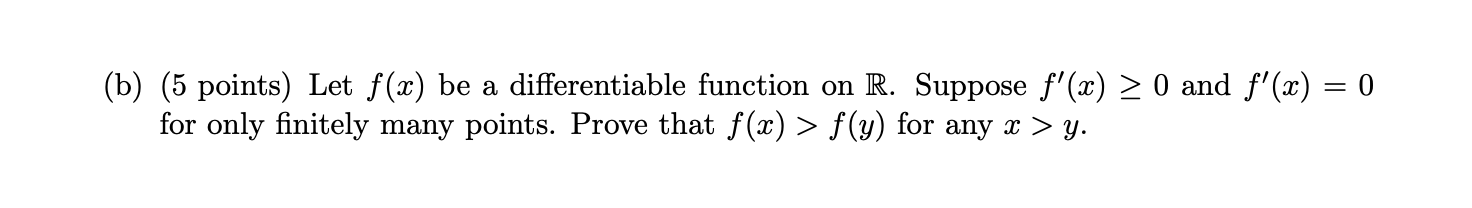
\includegraphics[width=400pt]{analysis--berkeley-104-final-46db.png}
\begin{proof}
  Let $y < x$ and suppose for a contradiction that $f(x) < f(y)$. Then from the mean value theorem we have that
  there exists $y < \alpha < x$ such that $f'(\alpha) = \frac{f(x) - f(y)}{x - y} < 0$. But this is a
  contradiction since $f'(x) \geq 0$ by supposition.

  Now suppose for a contradiction that $f(x) = f(y)$. Then the following procedure constructs infinitely many
  points $\alpha$ at which $f'(\alpha) = 0$:

  \begin{enumerate}
  \item Set $b = x$.
  \item Then by MVT there exists $\alpha \in (y, b)$ such that $f'(\alpha) = \frac{f(b) - f(y)}{b - y} = 0$. Note
    that as above, $f(\alpha) < f(y)$ is impossible since it would imply that the gradient is negative at some
    point in $(y, \alpha)$ by MVT. Similarly, $f(\alpha) > f(y)$ is impossible since it would imply that the
    gradient is negative at some point in $(\alpha, x)$. Therefore $f(\alpha) = f(y)$.
  \item Set $b = \alpha$ and repeat.
  \end{enumerate}

  This contradiction proves that $f(x) \ne f(y)$ and therefore that $f(x) > f(y)$.
\end{proof}

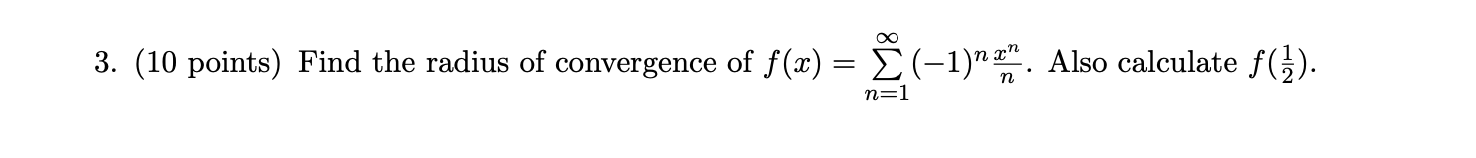
\includegraphics[width=400pt]{analysis--berkeley-104-final-4d1e.png}
\begin{proof}
  The series converges by the AST if $\Big|\frac{x^{n+1}}{n} / \frac{x^n}{n}\Big| < 1$ for all $n$.
  Since $\frac{x^{n+1}}{n} / \frac{x^n}{n} = x $ we have that the series converges if $|x| < 1$.

  \begin{align*}
    f(1/2)
    &= \sum_{n=1}^\infty (-1)^n \frac{1}{n2^n} \\
    &= -\frac{1}{2} + \frac{1}{2 \cdot 2^2} - \frac{1}{3 \cdot 2^3} + \frac{1}{4 \cdot 2^4} + \cdots \\
    &= \frac{1}{2}\Bigg( -1 + \frac{1}{2 \cdot 2^1} - \frac{1}{3 \cdot 2^2} + \frac{1}{4 \cdot 2^3} + \cdots \Bigg)
  \end{align*}



\end{proof}


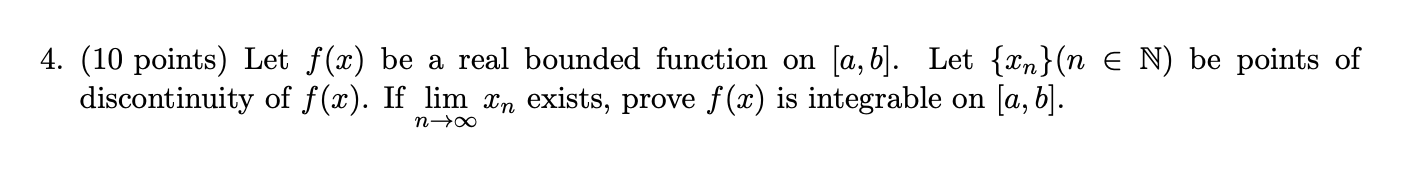
\includegraphics[width=400pt]{analysis--berkeley-104-final-48a9.png}




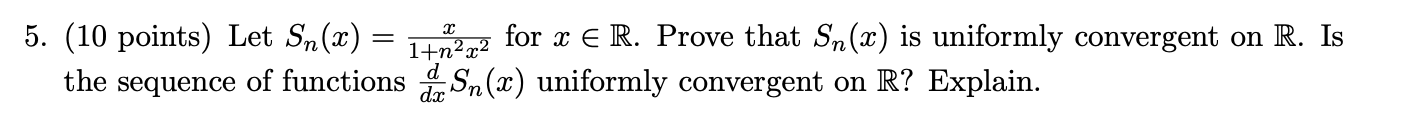
\includegraphics[width=400pt]{analysis--berkeley-104-final-f0c8.png}



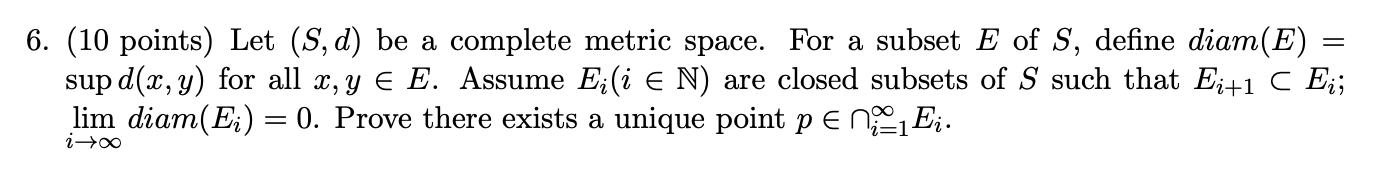
\includegraphics[width=400pt]{analysis--berkeley-104-final-bb9d.png}







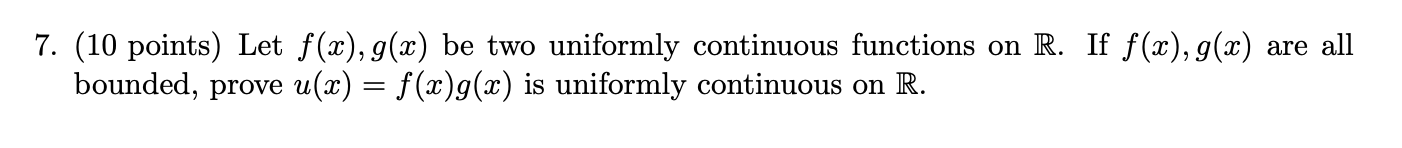
\includegraphics[width=400pt]{analysis--berkeley-104-final-5d66.png}



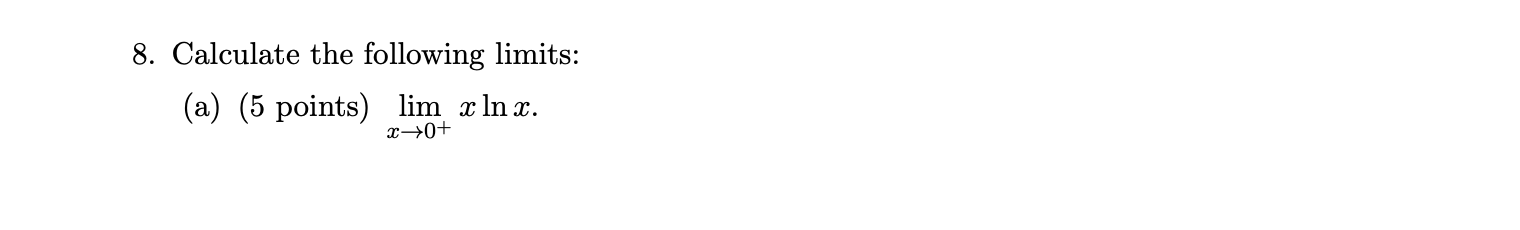
\includegraphics[width=400pt]{analysis--berkeley-104-final-9e97.png}





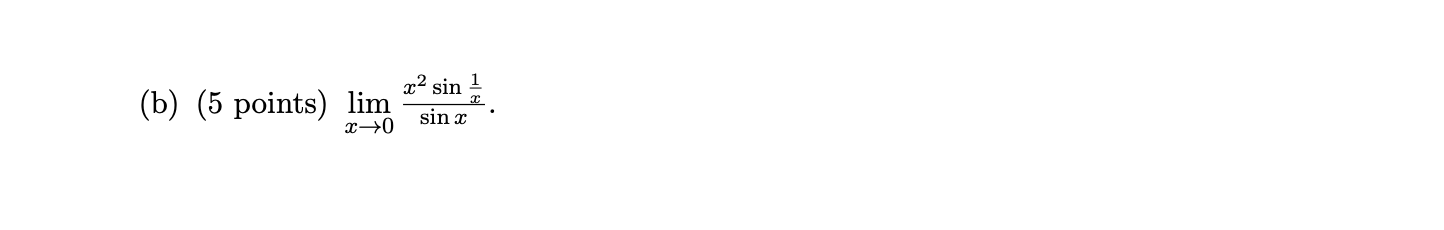
\includegraphics[width=400pt]{analysis--berkeley-104-final-763c.png}



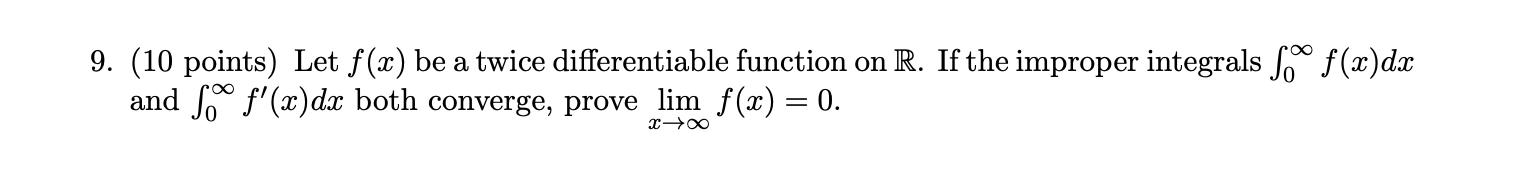
\includegraphics[width=400pt]{analysis--berkeley-104-final-e8fd.png}





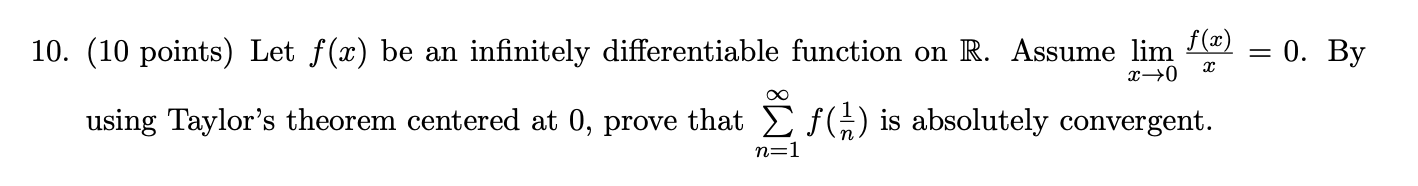
\includegraphics[width=400pt]{analysis--berkeley-104-final-b232.png}
